%!TEX encoding=UTF-8 Unicode
\chapter{Collecting Memory Traces}

Memory traces are useful to understand and optimize the memory usage of an application.
Still, collecting such a trace is challenging as there is no hardware help comparable to performance counters to do it non intrusively.
Therefore, memory trace collection tools must work at the \gls{OS} or software level.

In this chapter we present our main contributions that consists in two different memory trace collection tools.
The first tool, called \gls{Tabarnac}, uses an instrumentation library to obtain a global overview of the memory usage.
It is designed specifically to inspect \gls{NUMA} relate issues, has a low overhead and lock free design.
This tool also provides simple yet meaningful visualizations.
\gls{Tabarnac} was published at \gls{VPA} 2015 a \gls{SC} workshop~\cite{Beniamine15TABARNAC}.
Furthermore it is distributed as a free software under the \gls{GPL} license: \url{https://github.com/dbeniamine/Tabarnac}.
This work is the result of a collaboration with M. Diener and P.O.A Navaux from the informatica team of the \gls{UFRGS}, Porto Alegre, Brazil.
The second tool, \gls{Moca}, addresses the challenge of collecting \emph{complete} memory traces with temporal information.
It relies on an \gls{OS} level mechanism called page fault interception and injection.
This work is the subject of two Inria research reports~\cite{Beniamine15Memory,Beniamine16Moca} and has been submitted at \gls{PMBS} 2016, a \gls{SC} workshop.
As the previous tool, \gls{Moca} is distributed under the \gls{GPL} license: \url{https://github.com/dbeniamine/Moca}.

This chapter presents first the design and usage of \gls{Tabarnac} through a use case and discuss the obtain results and the limits in \sect{Tabarnac}.
Then we present the challenged raised \gls{Moca} and how it addresses them in \sect{Moca}.
Finally we provide an extensive comparison of our tools against state of the art memory trace tools in \sect{Tools-Comp}.


\section{Tabarnac: Global view of the memory usage}
\label{sec:Tabarnac}

\acrfull{Tabarnac} is our first attempt to collect memory traces and use them for performance optimizations.
As previous work~\cite{Beniamine13Cartographier} showed how difficult it is to capture \emph{complete} memory traces with temporal information, this tools focuses on the global behavior.
Furthermore it aims specifically at improving \gls{NUMA} related performance issues.

\subsection{Trace collection}

On \gls{NUMA} machines, optimizing memory performances often means reducing the number of remote accesses.
Indeed, to optimize the performances a memory page must be mapped to a physical memory bank as close as possible to the threads that actually uses it.
Remote accesses are extremely slow and must therefore be limited to the minimum possible.
Therefore to optimize memory performances on \gls{NUMA} system, it is required to know how much each page is accessed by each thread.
\acrful{Tabarnac} is designed to collect specifically this information.

\begin{algorithm}[htb]
    \begin{algorithmic}
        \Function{mem\_access}{unsigned long address, int threadId, char type}
            \State uint64\_t page = address >> page\_bits;
            \State accesses[threadId][page][type]++;
        \EndFunction
    \end{algorithmic}
    \caption{Handling of memory accesses by Tabarnac.}
    \label{alg:Tabarnac}
\end{algorithm}

\gls{Tabarnac} is based on Numalyze~\cite{Diener15Characterizing} instrumentation which rely on the \gls{Pin}~\cite{Luk05Pin} library.
This instrumentation is lock free by design: it traps on each memory accesses but only maintain two counters per pages and per threads, as details in \alg{Tabarnac}.
Numalyze was originally designed to estimate the efficiency of adaptive page mapping tools.
Indeed, such tools uses partial traces to decide online where to map memory pages.
Comparing the mapping obtained with a partial trace to the one obtained with the complete trace collected by Numalyze helps deciding the minimum size of partial trace required to decide on a page mapping.
We proposed to used theses traces for offline, interactive analysis.
Furthermore, as page number are not really meaningful for humans, we added contextual information to Numalyze traces.
Indeed, \gls{Tabarnac} also collects data structure information by three different means.
First, each time a thread is created, it compute its stack bounds and create a virtual structure named \texttt{Stack\#N} where $N$ is the thread~Id.
Then every time a binary file is loaded (main file or shared library), it inspect the binary, looking for static data structures.
Finally it intercept every call the \texttt{malloc} functions family, keeping track of data structures big enough.
Only structures that are bigger than one page (usually $4$Kib in current x86\_64 architectures) are recorded as our analysis granularity is the memory page. The data structure information (name, size and address) are only used to generate the visualization, after the end of the instrumentation.
The name detection of malloc'ed data structure is heuristic and based on source code analysis.

After tracing finishes, the tool generate three \texttt{csv} files.
The first contains the list of pages and the number of reads and writes per thread.
The second contains the list of structures with their names, sizes and start addresses, the last file contains the stacks size and addresses.
Then, a script which reads the trace, retrieves the page / data structure mapping and generates the final visualization presented in the next subsection.

\gls{Tabarnac} only depends on \gls{Pin} for the trace collection and \gls{R} for the visualization, and can be installed easily.
If all the R library required to generate the visualization are not present, it is able to install them automatically.
By default \gls{Tabarnac} generate the memory trace and the visualization, but the user can also choose to only generate the memory trace or the visualization.
This is useful for people who cannot install \gls{R} on the machine used to generate the trace.
Moreover it allows the user to customize the plots generate by the \gls{R} script.

\subsection{Visualization}

\begin{figure}[htb]
    \centering
    \begin{subfigure}{.49\linewidth}
        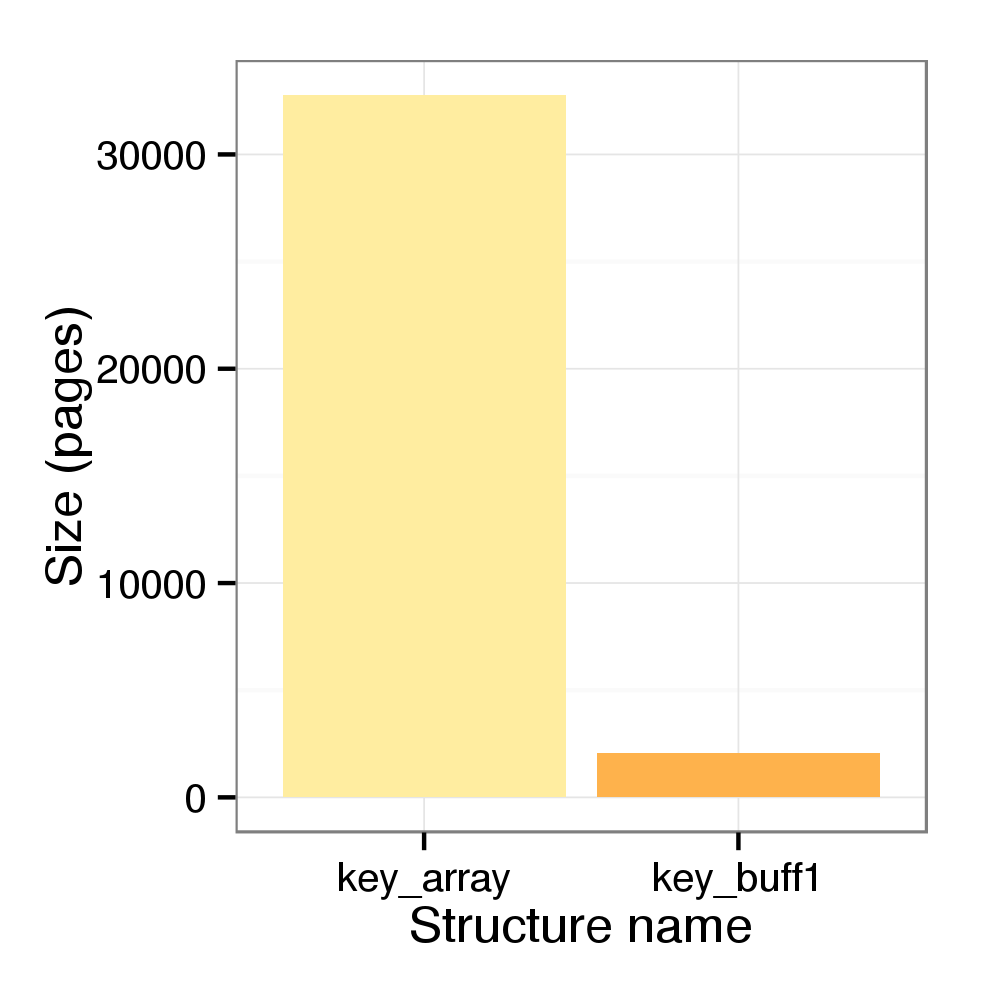
\includegraphics[width=\linewidth]{tabarnac/example_sz}
        \caption{Structures size.}
        \label{fig:example_sz}
    \end{subfigure}
    \begin{subfigure}{.49\linewidth}
        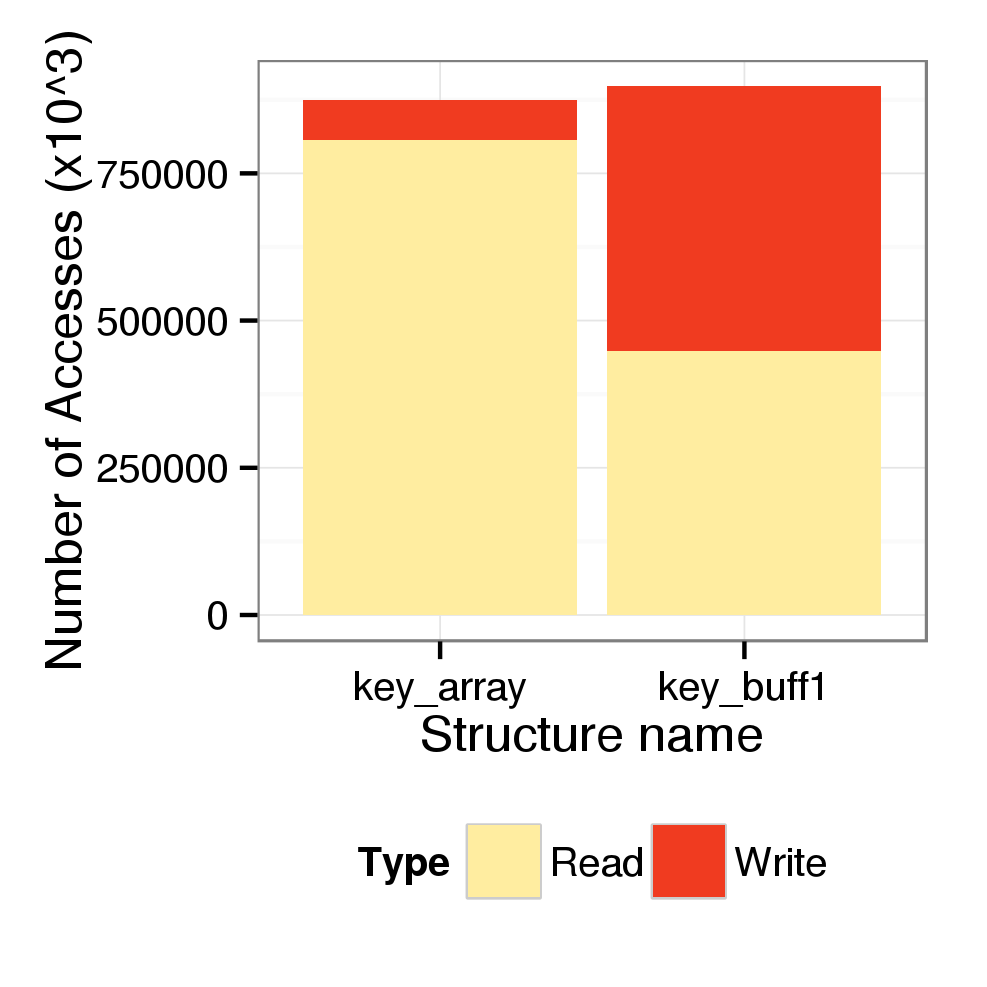
\includegraphics[width=\linewidth]{tabarnac/example_rw}
        \caption{Number of accesses per structures.}
        \label{fig:example_rw}
    \end{subfigure}
    \caption{Global views of the memory usage.}
    \label{fig:example_plot1}
\end{figure}

Once the data collection phase is done,
\gls{Tabarnac} generates the visualization (as an HTML page), providing a summary
of the trace through several plots\footnote{A full example of \gls{Tabarnac}'s output is available at:\\\small
    \url{http://dbeniamine.github.io/Tabarnac/examples}.}.
The visualization aims at showing \emph{why} performances issues related
to memory occur, it therefore shows several plots helping to understand the
importance of each data structure and how it is accessed.
Each plot is introduced by an explanation
of its presentation, what common issues it can help to understand and provides
suggestions on how to fix these issues.  The visualization starts with a small
introduction, summarizing the main principles while developing for NUMA
machines, and shows the hardware topology of the analyzed machine extracted
with Hwloc~\cite{Broquedis10hwloc}.


After the introduction, the visualization focuses on the usage of data structures. Some
structures are not displayed if less than $0.01\%$ of the total accesses happen on them. This is
done to make the output more readable by focusing on the most important structures.
%However, it is possible to ask
%\gls{Tabarnac} not to ignore structures in the second case for a more detailed view.

The first series of plots presents information concerning the relative
importance of the data structures. It consists of two plots, showing first the
size of each data structure, as in Figure~\ref{fig:example_sz}, then the
number of reads and writes in each structure (Figure~\ref{fig:example_rw}). These plots give a
general idea of the structures used by the parallel application.
Moreover, knowing the read/write behavior is very
useful as it determines the possible optimizations. For instance, structures
written only during initialization (or very rarely) can be relatively easily
duplicated, such that each NUMA node works on a local copy.

\begin{figure}[htb]
    \centering
    \begin{subfigure}{.49\linewidth}
        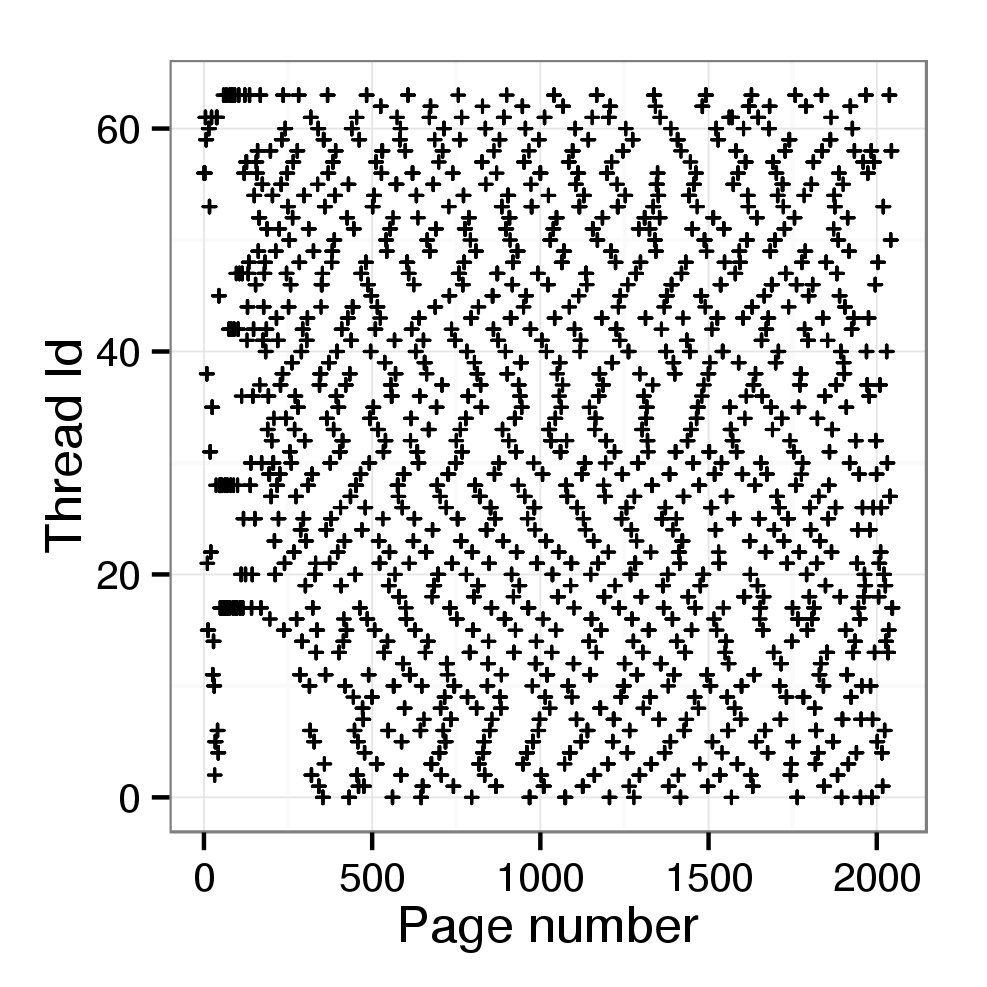
\includegraphics[width=\linewidth]{tabarnac/example_ft}
        \caption{First touch distribution.}
        \label{fig:example_ft}
    \end{subfigure}
    \begin{subfigure}{.49\linewidth}
        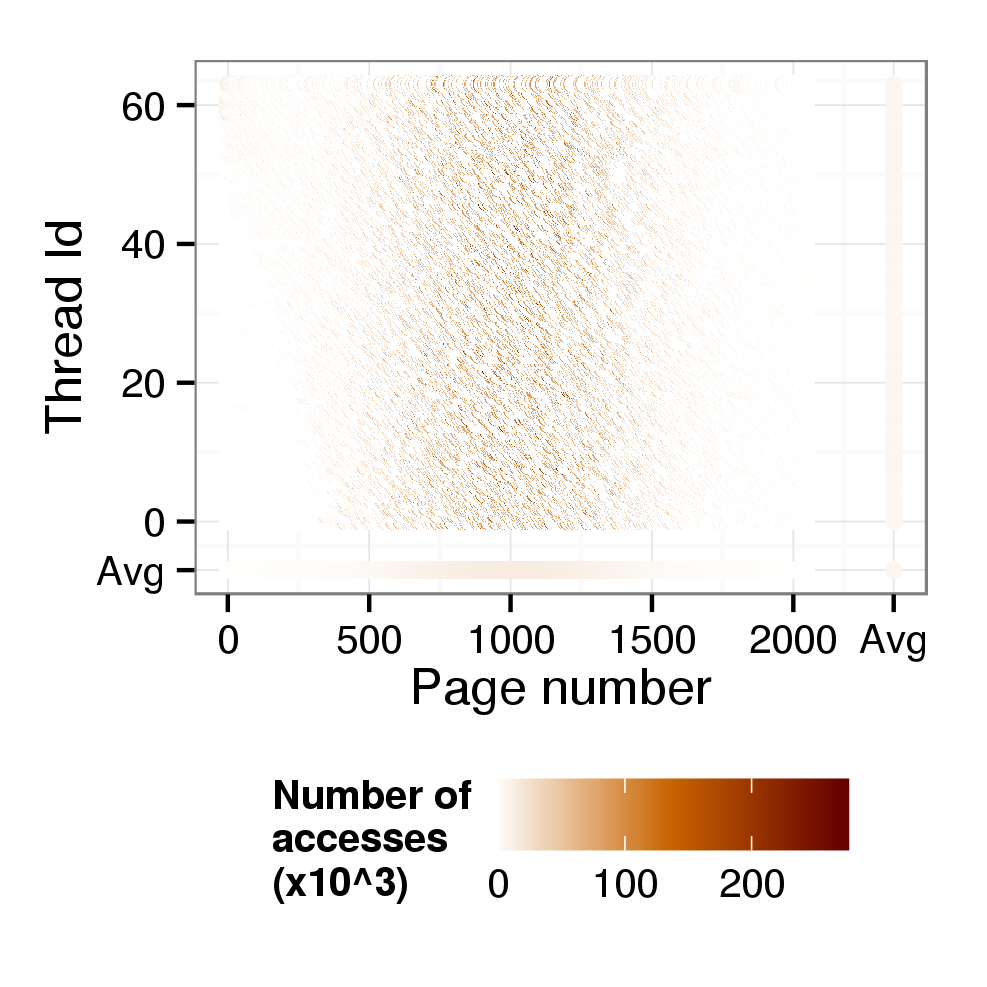
\includegraphics[width=\linewidth]{tabarnac/example_dist}
        \caption{Per thread access distribution.}
        \label{fig:example_dist}
    \end{subfigure}
    \caption{Per structure views.}
    \label{fig:example_by_structs}
\end{figure}

The second series of plots is the most important one. It
shows for each page of each structure
which thread was responsible for the first touch
(Figure~\ref{fig:example_ft}). This information is important as the
default policy for \emph{Linux} and most other operating systems is to map a page as close as possible to the first
thread accessing it. If the first touch distribution does not fit the actual
access distribution, the default mapping performed by \emph{Linux} might not be
efficient. To address this issue, the developer can either correct the first
touch or do some manual data mapping to ensure better memory access locality and balance
during the execution.

Finally, \gls{Tabarnac} shows the density of accesses performed by each thread and
the global distribution. In the example shown in Figure~\ref{fig:example_dist}, each
horizontal line represents the number of accesses to one page, there is one
line per thread and one for the average number of accesses. Moreover, for each
thread the average number of accesses to the structure is displayed.
Darker lines indicate more memory accesses to the page. This visualization gives an easy way
to understand the data sharing between threads, as well as the balance between pages and
threads. These plots can be used to identify inefficient memory access behaviors and to
determine the best NUMA mapping policy.

\subsection{Case study}

\Input{tabarnac-expe}


\section{Moca: Collecting fine grain traces}
\label{sec:Moca}

\subsection{Goals and challenges}

\DB{From Moca paper}

Some tools see the memory as a set of pages, loosing information at a finer
granularity. This approximation enable to trace memory accesses at a reduced
cost. For instance, \gls{Tabarnac}~\cite{Beniamine15TABARNAC} uses a binary
instrumentation (based on Intel's Pin~\cite{Luk05Pin}) and traps each
memory access, but it only keeps one counter per page and per threads in order to
reduce its overhead. While this approach provides a deeper insight about the
memory use than hardware performance counters, it lacks temporal information.





Finally, page faults interception can provide useful online information about memory usage.
Such a mechanism has been used in several existing works : in parallel garbage collectors~\cite{Boehm91Mostly}, in memory checkpointing~\cite{Heo05Spaceefficient} or in the domain of virtualization to provide the hypervisor with information about the memory usage of the guest \gls{OS}~\cite{Jones06Geiger}.
However, page faults only occur when caused by predetermined events in the system (copy-on-write, paging, ...).
Thus, just intercepting existing page faults only provide an approximate view of the memory use.
To improve this method, it is also possible to fake invalid pages at regular intervals in order to generate false page faults~\cite{Bae12Dynamic,Diener13CommunicationBased}.
 These false page faults are just triggered during regular memory accesses, that would not have caused a page fault if the page were not faked as invalid.
The advantage is that they create additional events for the monitoring tool to collect, thus more \emph{precision}, but the set of faked invalid pages has to be known and maintained by the monitoring tool.

As a final note, tools close to our proposal do not use false page faults injection and only need to store the location of memory pages and the threads that access them.
As a consequence, they require a relatively small data structure in memory for their own usage.
In this study we present \gls{Moca}, a new \emph{complete} memory trace collection system, based on page fault interception and false page faults injection, able to capture \emph{precisely} the temporal evolution of memory accesses performed by a multithreaded application.
To reach a satisfying \emph{precision}, our tool has to maintain in memory both the trace data and the set of faked invalid pages.
Overall, storing and exploiting efficiently these data within the kernel space and outputting them in real time to the user space is a challenge and is the main contribution of our work.



\subsection{Collection system design}

\subsection{Post processing}

\subsection{Moca validation}

\subsection{Discussion}

\section{Tools Comparison}
\label{sec:Tools-Comp}

\subsection{Tools analysis}

\subsection{Results and discussion}

\DB{Stuff from HPDC}

% vim: et si sta lbr  sw=4 ts=4 spelllang=en_us
